\section{Detector Efficiencies}
  To extract the electron-scattering cross section, one needs to know the number of scattered electrons coming out from the reaction plane (i.e. the target plane). Every detector is designed to be sensitive to certain types of particles within the known energy ranges. In practice, the detector may not be able to detect everyone of these particles passing through. Each detector has a detection efficiency ($\epsilon_{det}$) which is given as the portion of particles detected to the total. In addition, during the offline analysis, one applies cuts on the reconstructed quantities of the detectors to remove background and select good events, e.g. to identify pure electron events from the target. However, depending on the range of the cut, each cut may also unintentionally discard some good events. The cut efficiency ($\epsilon_{cut}$) denotes the percentage of good events remaining after applying a cut and has to be evaluated when one chooses the value of the cut. In other words, the detection efficiency denotes the survival rate of particles at the hardware level and the cut efficiency represents the level of confidence when selecting good particles at the software level, respectively. In this section, the efficiencies of the HRS detectors will be individually evaluated.

\subsection{Trigger Efficiency}
 The traditional HRS production trigger is generated by the coincidence of logic signals from two scintillator planes (S1 and S2m), so the trigger efficiency is equal to the product of the detection efficiency of these two scintillators. An inefficiency arises when either S1 or S2m does not fire when a particle passes through. As discussed in Section 3.7, T2 (T4) is the trigger generated when only one of S1 and S2m signals coincides with the gas \v{C}erenkov (GC) signal on HRS-R(-L). Using the events from T2 (T4), one can calculate the trigger efficiency of T1 (T3), or equivalently T6 (T7) in the E08-014, as follow: 
\begin{equation}
  \epsilon_{trig} = \frac{PS1(3)\cdot N_{T1(3)}}{PS1(3) \cdot N_{T1(3)}+PS2(4)\cdot N_{T2(4)}},
  \label{trigger_eff}
\end{equation}
where $N_{T1(2,3,4)}$ is number of events triggered by T1(2,3,4) and PS1(2,3,4) is the prescale factor of the trigger.

 Note that Eq.~\eqref{trigger_eff} is only valid when the GC has 100\% detection efficiency. Particles creating T1 (T3) Events ($N_{T1(3)}$) may not necessarily fire the GC, but events from T2 (T4) are recorded when the GC is fired, so $N_{T2(4)}$ has to be corrected by the detection efficiency of the GC. The trigger efficiency should be given by:
 \begin{equation}
  \epsilon_{trig} = \frac{PS1(3)\cdot N_{T1(3)}}{PS1(3) \cdot N_{T1(3)}+PS2(4)\cdot N_{T2(4)}/\epsilon^{GC}_{det}} 
  \label{trigger_eff2},
\end{equation}
where $\epsilon^{GC}_{det}$ is the detection efficiency of the GC. The HRS GCs usually have very high efficiency for detecting electrons, so Eq.~\eqref{trigger_eff} is still valid. However, when the efficiency of the GC falls, the trigger efficiency has to be corrected by the detection efficiency of the GC which is evaluated independently.

 In the E08-014, as the design of T1 and T3 involved S1, S2m and the GC, hence the trigger efficiency does not depend on the detection efficiency of the GC, which cancels in Eq.~\eqref{trigger_eff}:
 \begin{eqnarray}
 \epsilon_{trig} &=& \frac{PS1(3)\cdot N_{T1(3)}/\epsilon^{GC}_{det}}{PS1(3) \cdot N_{T1(3)}/\epsilon^{GC}_{det}+PS2(4)\cdot N_{T2(4)}/\epsilon^{GC}_{det}} \nonumber \\
                 &=& \frac{PS1(3)\cdot N_{T1(3)}}{PS1(3) \cdot N_{T1(3)}+PS2(4)\cdot N_{T2(4)}}.
  \label{trigger_eff3}
 \end{eqnarray}

 In summary, the assumption that the trigger efficiency is equivalent to the detection efficiency of S1 and S2m is valid only when both T1 (T3) and T2 (T4) involve the logic signal from the GC. 
\begin{figure}[!ht]
  \begin{center}
    \includegraphics[type=pdf,ext=.pdf,read=.pdf,width=0.9\textwidth]{./figures/scin/Trigger_Eff}
    \caption[Trigger efficiency vs run number]{\footnotesize{Trigger efficiency vs run number, where the top plot is for T3 trigger on HRS-L and the bottom plot is for T1 trigger on HRS-R.}}
    \label{trig_effi}
  \end{center}
\end{figure}
The trigger efficiencies of T1 and T3 were calculated individually for each run, shown in Fig.~\ref{trig_effi}. The results show that the triggers have very high efficiencies.

\subsection{Vertical Drift Chamber Efficiency}
 The detection efficiency of vertical drift chambers (VDCs) is usually very high and the inefficiency is mainly caused by the mis-reconstruction of particle tracks given by the tracking algorithm. Only events with one track were kept for the data analysis, and other events with zero-track and multi-tracks were discarded by applying a one-track-cut. The cut efficiency is generally called the one-track-cut efficiency, which is defined as:
\begin{equation}
  \epsilon_{vdc} = \frac{N_{Track=1}}{N_{0\leq Tracks\leq 4}},
  \label{eq_vdc_eff}
\end{equation}
where $N_{Track=1}$ is the number of events with only one track and $N_{0\leq Tracks\leq 4}$ is the number of events with tracks less than 4. Events with tracks more than 4 are extremely rare for HRS VDCs.

  To correctly evaluate $\epsilon_{vdc}$, good electrons were sampled by applying cuts on detector quantities. Those quantities that require tracking information were avoided when selecting electrons --- quantities derived from VDCs, the acceptance cuts on the focal plane and the target plane quantities, and the calorimeter's energy sum from the cluster reconstruction. Electrons can be alternately identified by cutting the calibrated ADC sums of the calorimeter and the GC. Events with multi-tracks can also be caused by multiple particles coming in one trigger window, and such events can be eliminated by requiring only one hit in each scintillator plane. Note that because paddles in S1 partially overlap, good events coming through the overlapped region are discarded when applying such a cut. This cut should be avoided for any other parts of data analysis.
  
 Cosmic ray events usually come into the VDC at large angles and give bad tracking reconstruction, and they can be eliminated by cutting on the time-of-flight velocity ($\beta_{TOF}$) calculated from the timing information from S1 and S2m. However, this information was not available in this experiment due to several nonfunctional TDC signals in S1 and S2m, so cosmic ray events were not removed. To suppress the cosmic ray background, data with high trigger rates, such as the carbon target data taken at the kinematic setting at the QE peak, were used to calculate the one-track-cut efficiency. From Table~\ref{vdc_table}, the fraction of one-track and multi-track events are listed, where the one-track efficiency is mostly above 99\%. The detection efficiency is the essential property of the detector and should not depend on the kinematic settings, hence one can conclude that the real value of the one-track-cut efficiency is equal to the values calculated with data taken at high rates.
\begin{table}[!ht]
  \centering
  \begin{tabular}{|c||ccccc|}
    \hline
    \textbf{Number of tracks}  & 0 & 1 & 2 & 3 & 4     \\
    \hline \hline
    HRS-L   & 0.030\% & 99.175\% & 0.743\% & 0.045\% & 0.005\%  \\
    \hline
    HRS-R   & 0.048\% & 99.360\% & 0.545\% & 0.039\% & 0.007\%  \\
    \hline 
  \end{tabular}
  \caption{Fraction of different tracks events from QE data,w/o $\beta$ cut}
  \label{vdc_table}	
\end{table} 
\subsection{Particle Identification Efficiencies}
 \begin{figure}[!ht]
  \begin{center}
    \subfloat[\footnotesize{Pion Rejectors}]{
      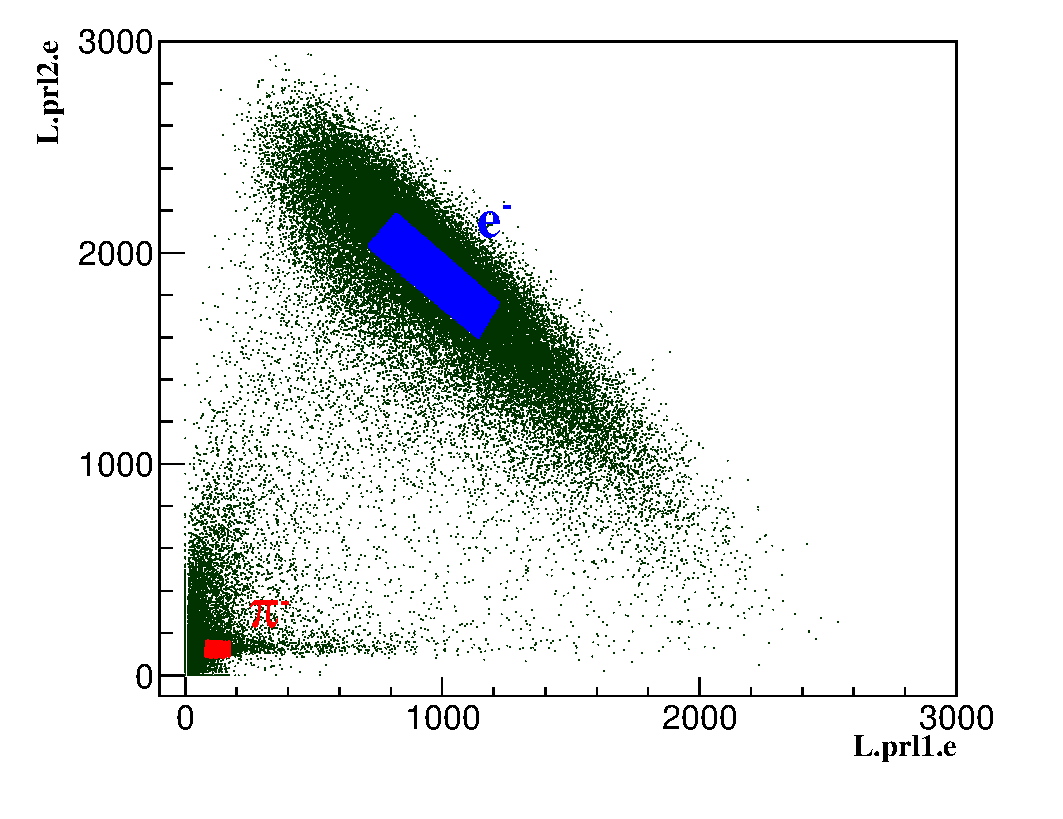
\includegraphics[type=pdf,ext=.pdf,read=.pdf,width=0.7\textwidth]{./figures/pid/L_PID_Calo.Cut_T7}
    }\\
    \subfloat[\footnotesize{Pre-Shower and Shower}]{
      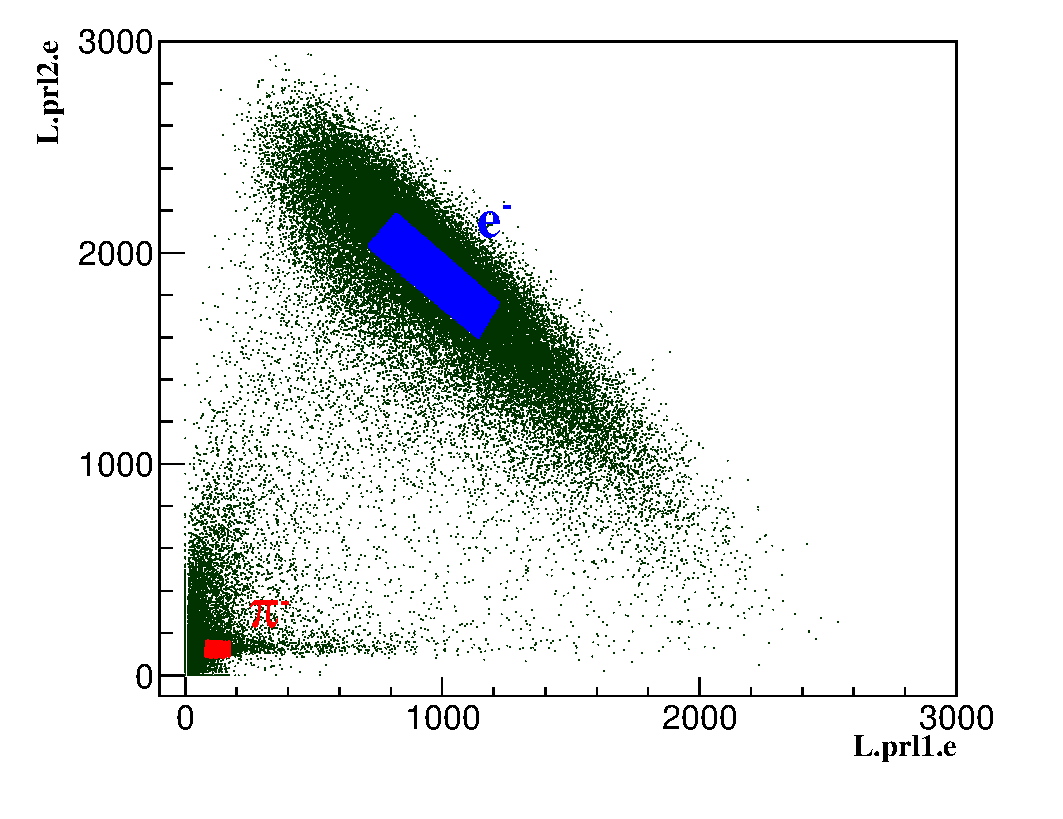
\includegraphics[type=pdf,ext=.pdf,read=.pdf,width=0.7\textwidth]{./figures/pid/L_PID_Calo.Cut_T7}
    }    
    \caption[Electron and pion samples from the calorimeters]{\footnotesize{Electron (blue) and pion (red) samples from the calorimeters. In each plot, the x-axis and the y-axis are the total energies collected by the first layer and the second layer of the calorimeter, respectively. Electrons create large signals either in the first or the second layer during the cascade while the signals created by pions are relatively small in each layer. Graphic cuts were applied on these regions (in color) to select the electrons and pions. } }
    \label{calo_sample}
  \end{center}
\end{figure}

 Electrons are identified by the GC and the calorimeter on each HRS. The GC gives high detection efficiency, since the momentum threshold for electrons to create \v{C}erenkov radiation is only 18 MeV/c, while pions and other heavy particles must have their momenta above 4 GeV/c to fire the detectors. The efficiency is mainly related to the performance of the mirrors in the GC to collect and focus the \v{C}erenkov light. 
\begin{figure}[!ht]
  \begin{center}
    \includegraphics[type=pdf,ext=.pdf,read=.pdf,width=1.00\textwidth]{figures/pid/Calo_E_P_Sample_Cer}
    \caption[Electron and pion samples from the GC]{\footnotesize{Electron and pion samples from the GC. The x-axis is the sum of calibrated ADC spectra of ten PMTs in the GC in HRS-L (top) or HRS-R (bottom). Electrons were selected by applying cut on the main peak of the spectrum. Pions can not directly create \v{C}erenkov light and they were selected by cutting on low ADC values.}} 
    \label{gc_sample}
  \end{center}
\end{figure}

 The detection efficiencies of the calorimeters are expected to be lower than the GCs. Each calorimeter is composed of many lead glass blocks, so the inefficiency arises when particles go through gaps between blocks or hit the edges of the calorimeter before it creates a shower. 
\begin{figure}[!ht]
  \begin{center}
     \subfloat[GC cut scan on HRS-L]{
      \includegraphics[type=pdf,ext=.pdf,read=.pdf,width=0.7\textwidth]{figures/pid/L_Cer_Cut_Eff_Geo_T7}
      } 
      \\
    \subfloat[GC cut Scan on HRS-R]{
      \includegraphics[type=pdf,ext=.pdf,read=.pdf,width=0.75\textwidth]{./figures/pid/R_Cer_Cut_Eff_Geo_T6}
      }
      \caption[Cut scan of the GCs]{\footnotesize{Cut scan of the GCs on HRS-L (top) and HRS-R (bottom). The x-axis is the channel number of the GC's ADC sum where the cut applies on. The cut efficiencies of pion (red boxes) and electrons (blue dots) were calculated with Eq.~\eqref{cut_eff_pi} and Eq.~\eqref{cut_eff_e} by varying the cut on the GC.} }
     \label{gc_cut_scan}
  \end{center}
\end{figure}

\begin{figure}[!ht]
  \begin{center}
     \subfloat[Calorimeter cut scan on HRS-L]{
      \includegraphics[type=pdf,ext=.pdf,read=.pdf,width=0.75\textwidth]{figures/pid/L_Calo_Cut_Eff_Geo_T7}
     } 
     \\
    \subfloat[Calorimeter cut scan on HRS-R]{
      \includegraphics[type=pdf,ext=.pdf,read=.pdf,width=0.75\textwidth]{./figures/pid/R_Calo_Cut_Eff_Geo_T6}
    }
     \caption[Cut scan of the calorimeters]{\footnotesize{Cut scan of the calorimeters on HRS-L (top) and HRS-R (bottom). The x-axis is the channel number of the calorimeter's ADC sum where the cut applies on. The cut efficiencies of pion (red boxes) and electrons (blue dots) were calculated with Eq.~\eqref{cut_eff_pi} and Eq.~\eqref{cut_eff_e} by varying the cut on the calorimeter.} }
     \label{calo_cut_scan}
  \end{center}
\end{figure}

 The particle identification (PID) for electrons was performed by applying cuts on the calibrated quantities of the GC and the calorimeter. The cuts can reject most unwanted particles, e.g. pions, but on the other hand, they may also accidentally discard good electrons. The PID study aims to obtain the optimized PID cuts on the GC and the calorimeter which can nearly eliminate pions while keeping as many electrons as possible. The cut efficiencies of the GC and the calorimeter have to be individually evaluated to correct the portion of electrons lost during the cuts. 
 
 To evaluate the detection efficiency of the GC (the calorimeter), one first selects electron samples from the calorimeter (the GC) and calculates the percentage of these samples being detected by the GC (the calorimeter), e.g. their signals are slightly larger than the pedestals in the ADC spectrum. Similarly, the evaluation of the cut efficiency for one detector also requires electron samples from the other detectors, but the cut applied on the signals of these samples should be significantly above the pedestals. Hence the calculation of the cut efficiencies for the GCs and the calorimeters should automatically include the detection efficiencies of these detectors.

 In general, for experiments with a large pion background, evaluating the percentage of residual pions mixed into the electron events ($\epsilon_{\pi}=1-\epsilon_{e-\pi}$) is also very crucial. However, compared with the electron rate in the QE region, the pion production rate during the E08-014 was very low. Additionally, the new trigger design had already removed most of pions during online data taking by introducing the GC in the trigger system. Hence the value of $\epsilon_{\pi}$ was expected to be very small. 
\begin{figure}[!ht]
  \begin{center}
    \subfloat[on HRS-L]{
      \includegraphics[type=pdf,ext=.pdf,read=.pdf,width=0.70\textwidth]{figures/pid/L_Cer_PID_Cut}
      \label{Lgc_eff}
    } 
    \\
    \subfloat[on HRS-R]{
      \includegraphics[type=pdf,ext=.pdf,read=.pdf,width=0.70\textwidth]{./figures/pid/L_Cer_PID_Cut}
      \label{Rgc_eff}
    }
    \caption[PID cut on the GCs]{\footnotesize{PID cut on the GCs. In each panel, the top and bottom histograms plot the calibrated ADC sum of events triggered by T1 (T3) and T6 (T7) from HRS-R (HRS-L), respectively. Most of pions have already been rejected in events from T1 and T3 during data taking, so a minimum cut on the GC's ADC spectrum ($\geq 50$) can further remove the rest of pions.}}
    \label{gc_eff}
  \end{center}
\end{figure}

 Events from the T6 and T7 triggers were used to study the PID cut efficiencies since they contained the most of pions. The VDC one-track-cut and the acceptance cuts were applied to select good events. Then pure pion samples and pure electron samples were chosen from the calorimeter (GC) when studying the cut efficiency of the GC (calorimeter). The pion~rejection~efficiency is defined as the percentages of pions removed by applying the PID cuts:
\begin{equation}
\epsilon_{\pi\_rej}^{GC(calo)} = \frac{N_{\pi}^{GC(calo)}}{N_{\pi\_samples}^{calo(GC)}}, 
\label{cut_eff_pi}
\end{equation}
  and the electron cut efficiency can be calculated from:
\begin{equation}
   \epsilon_{e\_cut}^{GC(calo)} = \frac{N_{e}^{GC(calo)}}{N_{e\_samples}^{calo(GC)}},
   \label{cut_eff_e}
\end{equation}
where $N_{\pi\_samples}^{calo(GC)}$ ($N_{e\_samples}^{calo(GC)}$) is the pion (electron) samples from the calorimeter (GC) (Fig.~\ref{calo_sample} and Fig.~\ref{gc_sample}). $N_{\pi}^{GC(calo)}$ is the number of pions rejected and $N_{e}^{GC(calo)}$ is the number of electrons left over after cutting on the GC (calorimeter), respectively. 
\begin{figure}[!ht]
  \begin{center}
    \subfloat[on HRS-L]{
      \includegraphics[type=pdf,ext=.pdf,read=.pdf,width=1.0\textwidth]{figures/pid/L_Calo_PID_Cut}
      \label{Lcalo_eff}
    } 
    \\
    \subfloat[on HRS-R]{
      \includegraphics[type=pdf,ext=.pdf,read=.pdf,width=1.0\textwidth]{figures/pid/R_Calo_PID_Cut}
      \label{Rcalo_eff}
    }
    \caption[PID cut on the calorimeters]{\footnotesize{PID cut on the calorimeters. Most of pions can be removed by the E/P cut ($E/P\geq 0.5$) and the cut on the second layer's ADC spectrum ($PRL2\geq 100$ or $SH\geq 200$).}}
    \label{calo_eff}
  \end{center}
\end{figure}

  A cut scan was performed to study the distributions of the pion rejection efficiencies and the electron cut efficiencies by varying the cuts on the GCs and the calorimeters, shown in Fig.~\ref{gc_cut_scan} and Fig.~\ref{calo_cut_scan}. Fig.~\ref{Lgc_eff} and Fig.~\ref{Rgc_eff} show that for the GC, a cut at the low channel value of the calibrated ADC sum, e.g. $\mathrm{L.cer.asum\_c\geq 50}$ for HRS-L or $\mathrm{R.cer.asum\_c\geq 50}$ for HRS-R, has already remove most of pions and preserve more than 99\% of electrons. The combined cuts on the calorimeter, $\mathrm{E/P\geq 0.5}$ and $\mathrm{L.prl2.e\geq 100}$ ($\mathrm{R.sh.e\geq 200}$), can further remove more than 90\% of pions while remaining more than 99\% of electrons, shown Fig.~\ref{Lcalo_eff} and Fig.~\ref{Rcalo_eff}. In total, on HRS-L (HRS-R), 99.85\% (99.62\%) of pions are eliminated with these combined PID cuts, while 99.58\% (99.86\%) of electrons survive after the cuts. Considering the high electrons rates and low pion production for this experiment, one is not required to specifically correct the pion contamination, and the value of $\epsilon_{e-\pi}$ in Eq.~\eqref{eqxs_org} was set to one.
